%%%%%%%%%%%%%%%%%%%%%%%%%%%%%%%%%%%%%%%%%%%%%%%%%%%%%%%%%%%%%%%%%%%%
%%%%%%%%%%%%%%%%%%%%%%%%%%%%%%%%%%%%%%%%%%%%%%%%%%%%%%%%%%%%%%%%%%%%
%%                                                                %%
%% An example for writting your thesis using LaTeX                %%
%% Original version by Luis Costa,  changes by Perttu Puska       %%
%% Support for Swedish added 15092014                             %%
%%                                                                %%
%% This example consists of the files                             %%
%%         thesistemplate.tex (versio 2.01)                       %%
%%         opinnaytepohja.tex (versio 2.01) (for text in Finnish) %%
%%         aaltothesis.cls (versio 2.01)                          %%
%%         kuva1.eps                                              %%
%%         kuva2.eps                                              %%
%%         kuva1.pdf                                              %%
%%         kuva2.pdf                                              %%
%%                                                                %%
%%                                                                %%
%% Typeset either with                                            %%
%% latex:                                                         %%
%%             $ latex opinnaytepohja                             %%
%%             $ latex opinnaytepohja                             %%
%%                                                                %%
%%   Result is the file opinnayte.dvi, which                      %%
%%   is converted to ps format as follows:                        %%
%%                                                                %%
%%             $ dvips opinnaytepohja -o                          %%
%%                                                                %%
%%   and then to pdf as follows:                                  %%
%%                                                                %%
%%             $ ps2pdf opinnaytepohja.ps                         %%
%%                                                                %%
%% Or                                                             %%
%% pdflatex:                                                      %%
%%             $ pdflatex opinnaytepohja                          %%
%%             $ pdflatex opinnaytepohja                          %%
%%                                                                %%
%%   Result is the file opinnaytepohja.pdf                        %%
%%                                                                %%
%% Explanatory comments in this example begin with                %%
%% the characters %%, and changes that the user can make          %%
%% with the character %                                           %%
%%                                                                %%
%%%%%%%%%%%%%%%%%%%%%%%%%%%%%%%%%%%%%%%%%%%%%%%%%%%%%%%%%%%%%%%%%%%%
%%%%%%%%%%%%%%%%%%%%%%%%%%%%%%%%%%%%%%%%%%%%%%%%%%%%%%%%%%%%%%%%%%%%

%% Uncomment one of these:
%% the 1st when using pdflatex, which directly typesets your document in
%% pdf (use jpg or pdf figures), or
%% the 2nd when producing a ps file (use eps figures, don't use ps figures!).
\documentclass[english,12pt,a4paper,pdftex,sci,utf8]{aaltothesis}
%\documentclass[english,12pt,a4paper,dvips]{aaltothesis}

%% To the \documentclass above
%% specify your school: arts, biz, chem, elec, eng, sci
%% specify the character encoding scheme used by your editor: utf8, latin1

%% Use one of these if you write in Finnish (see the Finnish template):
%%
%\documentclass[finnish,12pt,a4paper,pdftex,elec,utf8]{aaltothesis}
%\documentclass[finnish,12pt,a4paper,dvips]{aaltothesis}

\usepackage{graphicx}
\usepackage{epstopdf}

%% Use this if you write hard core mathematics, these are usually needed
\usepackage{amsfonts,amssymb,amsbsy,amsmath}

%% Use the macros in this package to change how the hyperref package below 
%% typesets its hypertext -- hyperlink colour, font, etc. See the package
%% documentation. It also defines the \url macro, so use the package when 
%% not using the hyperref package.
%%
%\usepackage{url}

%% Use this if you want to get links and nice output. Works well with pdflatex.
\usepackage{hyperref}
\hypersetup{pdfpagemode=UseNone, pdfstartview=FitH,
  colorlinks=true,urlcolor=red,linkcolor=blue,citecolor=black,
  pdftitle={Default Title, Modify},pdfauthor={Your Name},
  pdfkeywords={Modify keywords}}


%% All that is printed on paper starts here
\begin{document}

%% Change the school field to specify your school if the automatically 
%% set name is wrong
% \university{aalto-yliopisto}
% \university{aalto University}
% \school{Sähkötekniikan korkeakoulu}
\school{School of Science}

%% Only for B.Sc. thesis: Choose your degree programme. 
\degreeprogram{Mathematics and Systems Analysis}
%%

%% ONLY FOR M.Sc. AND LICENTIATE THESIS: Specify your department,
%% professorship and professorship code. 
%%
%\department{Department of Radio Science and Technology}
%\professorship{Circuit theory}
%%

%% Valitse yksi näistä kolmesta
%%
%% Choose one of these:
\univdegree{BSc}
%\univdegree{MSc}
%\univdegree{Lic}

%% Your own name (should be self explanatory...)
\author{Pasi Pyrrö}

%% Your thesis title comes here and again before a possible abstract in
%% Finnish or Swedish . If the title is very long and latex does an
%% unsatisfactory job of breaking the lines, you will have to force a
%% linebreak with the \\ control character. 
%% Do not hyphenate titles.
%% 
\thesistitle{Lattice Codes and Sphere Decoding}

\place{Espoo}

%% For B.Sc. thesis use the date when you present your thesis. 
%% 
%% Kandidaatintyön päivämäärä on sen esityspäivämäärä! 
\date{10.7.2017}

%% B.Sc. or M.Sc. thesis supervisor 
%% Note the "\" after the comma. This forces the following space to be 
%% a normal interword space, not the space that starts a new sentence. 
%% This is done because the fullstop isn't the end of the sentence that
%% should be followed by a slightly longer space but is to be followed
%% by a regular space.
%%
\supervisor{Prof.\ Camilla Hollanti} %{Prof.\ Pirjo Professori}

%% B.Sc. or M.Sc. thesis advisors(s). You can give upto two advisors in
%% this template. Check with your supervisor how many official advisors
%% you can have.
%%
%\advisor{Prof.\ Pirjo Professori}
\advisor{Prof.\ Marcus Greferath}
\advisor{D.Sc.\ Oliver Gnilke}
%\advisor{M.Sc.\ Polli Pohjaaja}

%% Aalto logo: syntax:
%% \uselogo{aaltoRed|aaltoBlue|aaltoYellow|aaltoGray|aaltoGrayScale}{?|!|''}
%%
%% Logo language is set to be the same as the document language.
%% Logon kieli on sama kuin dokumentin kieli
%%
\uselogo{aaltoRed}{''}

%% Create the coverpage
%%
\makecoverpage


%% Note that when writting your master's thesis in English, place
%% the English abstract first followed by the possible Finnish abstract

%% English abstract.
%% All the information required in the abstract (your name, thesis title, etc.)
%% is used as specified above.
%% Specify keywords
%%
%% Kaikki tiivistelmässä tarvittava tieto (nimesi, työnnimi, jne.) käytetään
%% niin kuin se on yllä määritelty.
%% Avainsanat
%%
\keywords{sphere decoding, space--time lattice codes, wireless communications}
%% Abstract text
\begin{abstractpage}[english]
 \end{abstractpage}

%% Force a new page so that the possible English abstract starts on a new page
%%
%% Pakotetaan uusi sivu varmuuden vuoksi, jotta 
%% mahdollinen suomenkielinen ja englanninkielinen tiivistelmä
%% eivät tule vahingossakaan samalle sivulle

\newpage

%% Preface
%%
%% Esipuhe 
%\mysection{Preface}


%\vspace{5cm}
%Otaniemi, 16.1.2015

%\vspace{5mm}
%{\hfill Pasi Pyrrö \hspace{1cm}}

%% Force new page after preface
%\newpage


%% Table of contents.
\thesistableofcontents


%% Symbols and abbreviations
\mysection{Symbols and abbreviations}

\subsection*{Symbols}

\begin{tabular}{ll}
$\mathbb{Z}$  & Set of integers \\
$\mathbb{C}$  & Field of complex numbers \\
$\mathbf{x}$  & Vector \\
$\mathbf{X}$  & Matrix \\
\end{tabular}

\subsection*{Operators}

\begin{tabular}{ll}
$\| \cdot \| $     & Euclidean norm \\
det$(\mathbf{X})$  & Determinant of matrix $\mathbf{X}$
\end{tabular}

\subsection*{Abbreviations}

\begin{tabular}{ll}
SNR & Signal to noise ratio \\
CVP & Closest vector problem
\end{tabular}


%% Tweaks the page numbering to meet the requirement of the thesis format:
%% Begin the pagenumbering in Arabian numerals (and leave the first page
%% of the text body empty, see \thispagestyle{empty} below).
%% Additionally, force the actual text to begin on a new page with the 
%% \clearpage command.
%% \clearpage is similar to \newpage, but it also flushes the floats (figures
%% and tables).
%% There is no need to change these
%%
\cleardoublepage
\storeinipagenumber
\pagenumbering{arabic}
\setcounter{page}{1}


%% Text body begins. Note that since the text body
%% is mostly in Finnish the majority of comments are
%% also in Finnish after this point. There is no point in explaining
%% Finnish-language specific thesis conventions in English. Someday 
%% this text will possibly be translated to English.
%%
\section{Introduction}
%% Leave first page empty
Wireless communication has been a crucial part of modern information technology for a couple of decades now. It is facing a lot of practical everyday problems which motivate the ongoing extensive research on the field. One of these problems is the noise and fading that occurs on wireless channels due to obstacles and radiation from the surroundings. To avoid data loss during transmission via wireless link one has to encode the data to be sent in such a robust way that it can still be recovered at the receiving end even in the presence of noise and fading of reasonable scale. 
\par One way to tackle this problem, and the method this thesis focuses on, is the use of space--time lattice codes and sphere decoding. From a mathematical point of view the process of decoding can then be viewed as a problem of finding the closest lattice point to a given input vector, that is, the possibly noisy vector containing the data we receive from the wireless channel. This problem in its general form is known to be NP-hard but for communications applications, where the dimensionality and lattice shape are kept reasonable, there exist algorithms, like the sphere decoder, that offer polynomial expected complexity \cite{mia}.


%% In a thesis, every section starts a new page, hence \clearpage
\clearpage

\section{Lattices in communications technology}

Before we go into communications applications of lattices such as lattice codes, let us start off with the definition of a lattice. Let $n$ and $m$ be positive integers such that $n \leq m$ and $\mathbf{b}_1, ... , \mathbf{b}_n \in \mathbb{R}^m$ be linearly independent vectors. A subset $\Lambda$ of $\mathbb{R}^m$ is called a lattice of dimension $n$ if it is defined as

\begin{equation}
\Lambda = \sum_{i=1}^{n} \mathbb{Z}\mathbf{b}_i = \{a_1\mathbf{b}_1 + ...+a_n\mathbf{b}_n | a_i \in \mathbb{Z}, 1 \leq i \leq n\}\label{eq:lattice}
\end{equation}

\noindent where the set of vectors $\mathbf{b}_1, ... , \mathbf{b}_n \in \mathbb{R}^m$ is called the basis of the lattice $\Lambda$. All points of the lattice can be obtained as a linear combination of the basis vectors $\mathbf{b}_i$ and integer coefficients $\mathbf{a}_i$ as stated in \eqref{eq:lattice}. The number of basis vectors $n$ is also called the rank of the lattice and if $n = m$ the lattice is said to have full rank. The points of the lattice $\Lambda$ form a group under addition which means that if $\mathbf{x} \in \Lambda$ then $-\mathbf{x} \in \Lambda$ and if $\mathbf{x}, \mathbf{y} \in \Lambda$ then $\mathbf{x} \pm \mathbf{y} \in \Lambda$. \cite{cassels}
\par There is also a matrix representation for the same lattice
\begin{equation}
\Lambda = \{\mathbf{x}|\mathbf{x} = \mathbf{B}\mathbf{a} \} \label{eq:matrix}
\end{equation}
where $\mathbf{B} = [\mathbf{b}_1, ... , \mathbf{b}_n]$ is an $m \times n$ matrix called the generator matrix of the lattice $\Lambda$ and $\mathbf{a}$ is an $n$-dimensional integer column vector. Note that $\mathbf{B}$ is not uniquely determined by the lattice as in fact there exists infinitely many bases for the same lattice \cite{cassels}. If $\mathbf{B}$ is a basis for lattice $\Lambda$ then $\mathbf{B}'$ is also a basis for the same lattice if the following holds
\begin{align}
\mathbf{B}' &= \mathbf{W}\mathbf{B}, \\
\text{det}(\mathbf{W}) &= \pm 1
\label{eq:basis_change}
\end{align}
where $\mathbf{W}$ is an $m \times m$ matrix with integer entries \cite{agrell}. Some bases are however better in some sense than others, especially in communications applications, as one could imagine. Usually reasonable orthogonality and relatively small norm for the basis vectors are desired \cite{agrell}. A better basis can be obtained via a process called basis reduction, which is illustrated in figure \ref{fig:bases}. Clearly basis vectors $\mathbf{u}_i$ obtained from the basis reduction are more pleasant to work with than the original vectors $\mathbf{v}_i$ although they both span the same lattice.

\begin{figure}[ht]
  \centering
  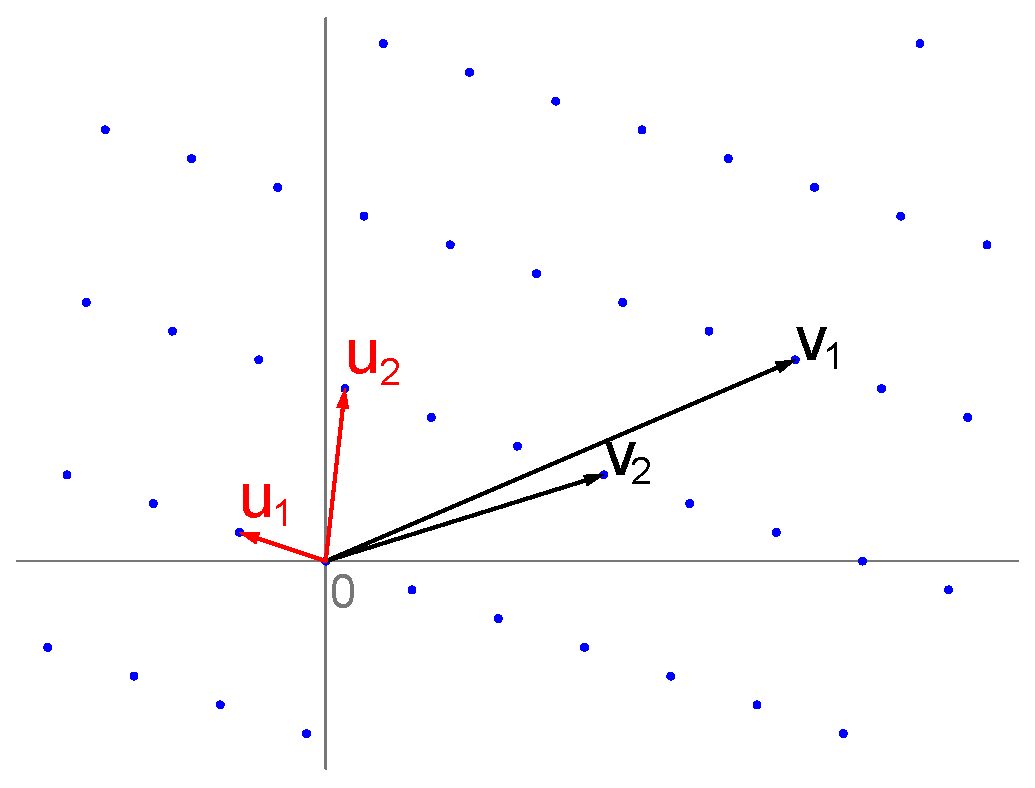
\includegraphics[width=0.8\linewidth]{Lattice-reduction}
  \caption{Two different bases for the same two dimensional lattice.}
  \label{fig:bases}
\end{figure}

\par What we considered earlier were lattices spanned over real $m$-dimensional space $\mathbb{R}^m$ but in similar sense we can consider a lattice consisting of complex valued vectors from $\mathbb{C}^m$. The principles of such complex lattice are almost the same, however, now $\mathbf{B}$ and $\mathbf{a}$ take values from $\mathbb{C}$. Note that a complex lattice has an equivalent real representation which has double the rank of the corresponding complex lattice. Consider a lattice $\Lambda \subset \mathbb{C}^m$ with a generator matrix $\mathbf{B} = [\mathbf{z}_1, ... , \mathbf{z}_n]$. Now we can always express it with a real valued lattice $\Lambda_{\text{real}} \subset \mathbb{R}^{2m}$ and the corresponding $2m \times n$ generator matrix is given by

\begin{equation}
\mathbf{B}_{\text{real}} =
\begin{bmatrix} 
\text{Re}(z_{11}) & \dots  & \text{Re}(z_{1n}) \\
\text{Im}(z_{11}) & \dots  & \text{Im}(z_{1n}) \\
\vdots            & \ddots & \vdots            \\
\text{Re}(z_{m1}) & \dots  & \text{Re}(z_{mn}) \\
\text{Im}(z_{m1}) & \dots  & \text{Im}(z_{mn}) \\
\end{bmatrix}.
\label{eq:complex}
\end{equation}
In other words we convert each column of $\mathbf{B}$ to real vector by separating each of their complex elements into two adjacent real elements, that is the real and imaginary parts of the original complex element. This process doubles the amount of rows in $\mathbf{B}_{\text{real}}$ but both representations ultimately describe the same lattice. \cite{conway}

\subsection{Closest vector problem}

One relevant mathematical problem related to sphere decoding, a communications application of interest in this paper, is the closest vector problem (CVP). Given a lattice $\Lambda$ and an input point $\mathbf{y}$ the problem is to find a lattice point $\hat{\mathbf{x}} \in \Lambda$ that is closest to $\mathbf{y}$. More precisely $\hat{\mathbf{x}} \in \Lambda$ has to meet the following condition

\begin{equation}
\|\mathbf{y}-\hat{\mathbf{x}}\| \leq \|\mathbf{y}-\mathbf{x}\|, \ \ \ \forall \mathbf{x} \in \Lambda.
\label{eq:cvp}
\end{equation}

\noindent For a fixed point $\hat{\mathbf{x}} \in \Lambda$ the set of vectors $\mathbf{y}_i$ that satisfy the confition \eqref{eq:cvp} is called the Voronoi region of lattice point $\hat{\mathbf{x}}$, $\mathcal{V}_{\hat{\mathbf{x}}}$. This means that if $\mathbf{y} \in \mathcal{V}_{\hat{\mathbf{x}}}$ then the solution to CVP is $\hat{\mathbf{x}}$. The volume of the $\mathcal{V}_{\hat{\mathbf{x}}}$ is given by det$(\Lambda) = $ $\sqrt{\text{det}(\mathbf{B}^T\mathbf{B}})$, where $\mathbf{B}$ is the generator matrix of $\Lambda$.

\subsection{Space--time lattice codes}

\clearpage

\section{Sphere decoder}

\clearpage

\section{Simulations and results}
 
\clearpage

\section{Summary}


\clearpage
%% L\"ahdeluettelo
%%
%% \phantomsection varmistaa, ett\"a hyperref-paketti latoo hypertekstilinkit
%% oikein.
%%
%% The \phantomsection command is nessesary for hyperref to jump to the 
%% correct page, in other words it puts a hyper marker on the page.

\phantomsection
\addcontentsline{toc}{section}{\refname}
%\addcontentsline{toc}{section}{References}
\begin{thebibliography}{99}

\bibitem{mia} Mäki,\ M. \textit{Space-time block codes and the complexity of sphere decoding.} Doria, Referenced 10.7.2017. Available:
  \url{https://www.doria.fi/bitstream/handle/10024/54404/gradu2008maki-miia.pdf}
  
  
\bibitem{cassels} Cassels, J.W.S. \textit{An introduction to the Geometry of Numbers}, New York, Springer--Verlag, 1971.

\bibitem{agrell} Agrell, E., Eriksson, T. and Zeger, K. \textit{Closest point search in lattices} IEEE Transactions on Information Theory, Vol. 48, pp.2201-2214,
August 2002.

\bibitem{conway} Conway,\ J.H. and Sloane,\ N.J.A. \textit{Sphere packings, lattices and groups.} Third edition, New York, Springer--Verlag, 1998.


\end{thebibliography}

%% Appendices
%% Liitteet
\clearpage

\thesisappendix


\end{document}
